\chapter{Probabilistic dynamic security assessment}
\label{ch:DPSA}
\minitoc

Need more data than deterministic. It should be noted that, even if using more complex models, the exact value of the risk (in MWh/y or €/y) is of low significance. What is important is to be able to compare the risk associated with different scenarios and to be able to identify actions that most effectively reduce the risk.

PDSA will provide useful information even with garbage data, but better data gives better results \url{https://xkcd.com/2295/} ('Garbage In, Garbage Out' should not be taken to imply any sort of conservation law limiting the amount of garbage produced.)

Limit analysis to short-term stability for sake of simplicity, but could be applied to long-term too (or both, Eurostag, Dynawo)

\TODO{ML figure: coverage, importance, historical}

\TODO{Show more the ximple windows than in paper (e.g. likelyhood of a contingency having consequcens, etc.)}

\TODO{Mention missing trips (other than fault clearing)}

\TODO{Use the DPSA acronym. Potentially distinguish between DPSA and probabilistic DSA}

\TODO{Explain the choice of considered failure modes: EHV faults most likely to causes wide-area issues, EHV protected by diff+distance (in Elia) and talks for double diff, diff is a very good protection, cannot really be misconfigured and self-testing of relays (incl. more advanced stuff like Russian paper in CIGRE 2022 proceedings)}

\TODO{(D)PSA is more of a process than a methodology, refine the models/data by iteration}

\TODO{Curse of dimensionality / peel, example with hypersphere}

\TODO{Bien situer le contexte (vision planing mais opérationel envisable avec modifications), ce qui existe déjà, etc.}

Limit analysis to short-term stability for sake of simplicity, but could be applied to long-term too (or both, Eurostag, Dynawo), same for ch 6

\TODO{Protection indicator helps a bit with coverage, although don't know how much}

The objective of a probabilistic security assessment are to list the possible accident scenarios that can lead to unwanted consequences, to estimate the probability of these scenarios, and to estimate their consequences. Such assessment can be decomposed into two parts: (i) listing (or sampling) the possible pre-contingency states, and (ii) determining the possible post-contingency evolutions. As highlighted in the literature review (section~\ref{sec:probabilisticSecurity}), the second part is actually the hardest.

In a deterministic approach, only one post-contingency evolution is considered, because one assumes that all transmission equipment and protection systems operate as expected. The evolution is computed by simulation. Often, the protection systems are not explicitly modelled in the simulation. Their effect (e.g. fault clearing by opening a line) is predicted in advance and included in the simulator as part of the contingency. In a probabilistic approach, possible misoperations are considered which leads to multiple possible system evolutions. One way to handle those multiple possible evolutions is to use event trees as done in~\cite{Haarla, GridPSA}. Event trees are presented in section~\ref{sec:DynMethods} and in Figure~\ref{fig:eventTree}. In the approach proposed in~\cite{Haarla, GridPSA}, event trees are built prior running simulations. So, only events that can easily be predicted without simulations can be included\footnote{For example, if the initiating event is a line fault, the events that can easily be predicted are the triggering of the protections of this line, and their backup protections.}. Another limitation of event trees is that event are placed in a so-called event axis instead of a time axis. So, it is assumed that the timing of events does not influence the evolution of the system.

In theory, a skilled analyst can alleviate the above limitations. He can use his expertise and/or simulation results to identify events that can occur during the system evolution. Also, if the order and/or timing of events is of importance, he can add additional events to consider them (e.g. split ``event A occurs" in ``events A occurs before \(t=\)~5~s" and ``event A occurs after \(t=\)~5~s). It can however be difficult to compute the probabilities associated with those events. Also, the analyst should try to only consider the most critical scenarios to avoid an explosion of the size of the tree. So, in practice, this requires a lot of effort from the analyst. So-called dynamic event trees (DETs) have thus been developed with the objective to move most of the burden of proof of correctness from the analyst to the methodology. DETs are introduced in section~\ref{sec:dynamicReliability}.

It should however first be noted while the above observations have mostly been made in the nuclear sector (wherefrom event trees originated)~\cite{LabeauTowards}, they are even more relevant for power systems. There is two main reasons for this. First, there are significantly more initiating events to consider. Indeed, one should consider at least hundreds of possible (e.g. line) faults or even more depending on the size of the considered system (and the voltage level(s) considered). Also, for a given fault, multiple event trees should be built as the evolution of the system depends on the initial operating conditions. Second, a large number of events can occur after a disturbance, especially during fast cascading outages. Predicting those events as well as determining the importance of the timing and order of events might prove particularly complex.

Section~\ref{sec:dynamicReliability} introduces DETs and reviews the literature on the subject. Section~\ref{sec:proposedMethodology} discusses the proposed methodology. Section~\ref{sec:DataRequirementsForDSA} discusses the data requirements for dynamic probabilistic security assessment, and section~\ref{sec:testCases} presents the test cases used.


\section{Dynamic reliability methods}
\label{sec:dynamicReliability}

\textbf{Note:} In the final thesis, this section will introduce more rigorously DETs and the different techniques that can be used to solve them. Also, ``dynamic reliability" techniques (that include DETs) will be reviewed. In this report, only MCDET, the specific DET solving technique used in this work, is presented.

A DET follows the (time-dependant) evolution of the system after a given initiating event. This tree branches each time the system can transition to different states. For example, if the initiating event is a line fault, the DET will branch at the times when each of the circuit breakers (CBs) open. In that case, each branch is associated with a possible state of the CBs (i.e. both open, both closed or one open and one closed) and follows the evolution of the system in that given state. Additionally, because the operating time of the circuit breakers is not known with an infinite precision, branchings are made at each point in time were the breakers are likely to operate. If CB opening times are assumed to follow some continuous probabilistic distribution, there is theoretically an infinity of possible branching points to consider. Techniques are thus needed to solve them numerically.

It should be noted that contrarily to ``static" event trees, branching points are not defined explicitly but via branching rules. For example, if the line is protected by distance protection scheme, the relays and CBs should be included in the model. Then, during the system evolution, when the apparent impedance seen by a relay goes below a (potentially uncertain) threshold, the relay send a tripping signal to the CB that either opens (after an uncertain amount of time) or fails to open. Branches are automatically created to follow the possible system evolutions (e.g. CB fail to open, CB opens 60~ms after receiving the signal, CB opens 80~ms after receiving the signal, etc.).

One of the available techniques is MCDET. MCDET is a concatenation of MC (Monte Carlo) and DDET (discrete DET). In MCDET, continuous uncertainties (e.g. threshold values, CB opening delays) are handled by MC and discrete uncertainties (e.g. CB fails to open) are handled by DDETs. DDETs are based upon the restriction of the possible branching points to discrete points in time. In other words, the system evolution after a disturbance is simulated, and at each time step branchings are created following aforementioned branching rules. The drawback of DDETs is the combinatorial explosion of the number of branches (that grows as the average number of branches created at each step to the power of the number of steps). To manage this explosion, it is necessary to introduce cutoffs (e.g. do not follow branches that have a probability lower than a threshold) and to increase the size of the time steps. It is however difficult to estimate how the size of the time steps and the cutoff thresholds affect the accuracy of the DET solving method. So, it is difficult to make a good compromise between accuracy and computation time.

In MCDET, a DDET is built for each (MC) sample of the continuous uncertainties. As only discrete uncertainties have to be handled by the DDETs, they can potentially be built completely (i.e. with no cutoffs and a very small time step). In this case, the accuracy of the DET solving technique depends only on the MC part. This is convenient as MC accuracy can be estimated easily with statistical methods.


\section{Proposed methodology}
\label{sec:proposedMethodology}

As discussed in the previous section, the security assessment method used in this thesis is based on MCDET. An additional element has however to be added to the methodology to properly model the pre-disturbance state of the grid. Indeed, given a particular realisation of generator and transmission asset availabilities and load, system operators will try to dispatch power plants to minimise total costs while maintaining acceptable operating conditions (e.g. no overloads, acceptable voltages, etc.). The optimisation problem associated is called an optimal power flow (OPF). When potential (usually N-1) contingencies are considered, this is referred to as a security constrained (SC) OPF.

The methodology can thus be summarised as follow. First, generate a sample of the pre-contingency state (i.e. availability of assets, renewable production, etc.) and consolidate it by running a (SC)OPF program. Then, sample the remaining continuous uncertainties. Build a DDET to handle the discrete uncertainties. Repeat the above procedure until statistical convergence.

\TODO{Simplified model of a few steps of slow cascade?}
% \TODO{Mention forecasting errors for the SCOPF? (not considered in the thesis)}
\TODO{(Foot)note: sampling protection threshold before simulation implies ``tabou" region~\cite{Faghihi}.}


\section{Data requirements for dynamic probabilistic security assessment}
\label{sec:DataRequirementsForDSA}

Dynamic probabilistic security assessment requires a large amount of input data. The following paragraphs thus discuss the data needed to model the pre-disturbance state, the disturbances themselves, and the post-disturbance evolution.

\subsection{Pre-disturbance state}

The data required to model the pre-disturbance state of the grid is quite similar to the one used in deterministic dynamic security assessment (that is discussed e.g. in~\cite{EurostagHPC}). These data consist mainly of generation and load forecasts for the considered period. Planned maintenances are also often included. In a probabilistic assessment, the only additions could be unplanned maintenances and forecast errors. These are not considered in this thesis. Finally, the (SC)OPF also requires some data: running costs of generators (or at least a merit order) and static (current) limits.

\subsection{Disturbances}

In a probabilistic assessment, it is of course necessary to estimate the frequency of occurrence of disturbances. This requires historical statistics of past disturbances.

\subsection{Post-disturbance evolution}

Modelling the post-disturbance evolution of a system in a probabilistic assessment is generally more complex than in a deterministic one. This is because, in a probabilistic analysis, the system has to be simulated further away from normal operation (e.g. during cascading outages). For this, one should generally model the generators (including governors and voltage regulators), loads, transformers, etc. with the best (RMS) models available. If the accuracy of a model is deemed insufficient (e.g. difficulty to reproduce past disturbances, high sensitivity to input data, etc.), then better models have to be developed and/or better data have to be collected.

Additionally, since the system is simulated in degraded states, protections have to be modelled explicitly\footnote{At least, the protections that are discussed in chapter~\ref{ch:protections}.}. This requires to know what protections are installed in the system and what are their settings. Finally, to compute the frequency of scenarios, it is necessary to have an estimate of the probability of failure of protection systems. It is best to also have probability density functions (pdfs) of the protections thresholds\footnote{In order to model measurement and setting errors. The second point is particularly challenging.} and operating times. Pdfs of all aforementioned parameters can also be used to refine the analysis and perform sensitivity studies.

\TODO{2-3 mots sur ce qu'Eurostag appèle le modèle electromec étendu (p117)}

\section{Test cases}
\label{sec:testCases}

The method proposed in this thesis will be applied on a variety of test cases. This report present two of them: the Roy Billinton test system (RBTS) and the three-area reliability test system (RTS). They are shown in Figure~\ref{fig:rbts-ch6} and~\ref{fig:rts} respectively. These systems were chosen because they include part of the necessary data (static data, load and generation profiles\footnote{The grid modernization laboratory consortium (GMLC) developed an updated version of the RTS. This version has a significant installed capacity of renewable generation. It also mapped the system to a geographical area such that meteorological data can be used to generate coherent generation forecasts.}, economic data). Missing data include dynamic data (i.e. generator models) and protection data (types of protection installed, settings and reliability data). Another criterion in the choice of these systems is their size. The RBTS is a small (6-bus) system that can be used in simple case studies and for debugging. The RTS is a medium (73-bus) system that is large enough to represent cascading mechanisms found in larger grids, yet not to large which eases the interpretation of results, data handling and computational issues\footnote{Finally, those systems were developed for research on reliability. Contrarily to other systems, parallel lines and parallel generators are not replaced with equivalent elements. This allows to more easily perform N-1 security analysis (double line failures are not accidentally considered as N-1 contingencies) and fill the missing data (generators have more realistic sizes, so typical parameters are easier to find).}.

\begin{figure}
    \centering
    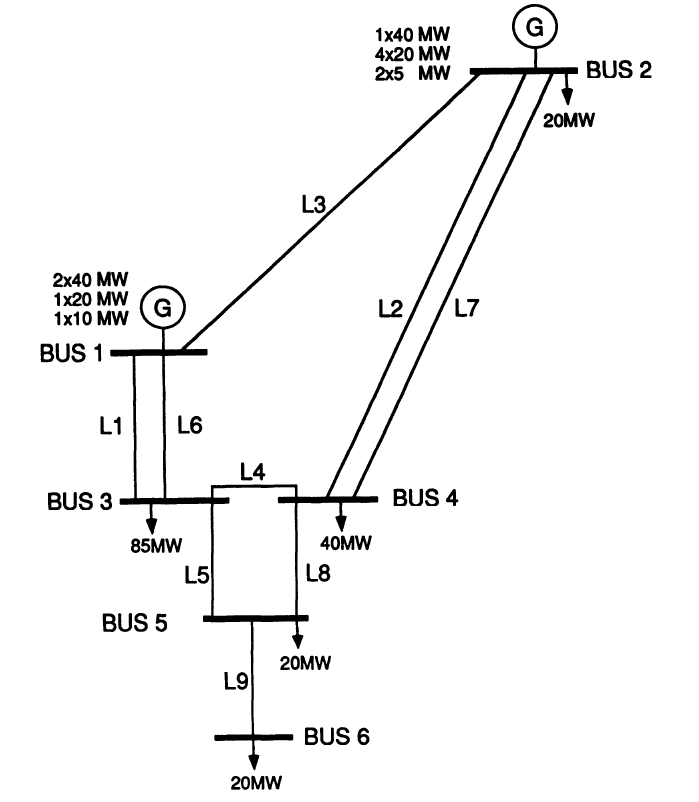
\includegraphics[width=0.6\linewidth]{Figs/RBTS.png}
    \caption{Roy Billinton test system. Adapted from~\cite{rbts}}
    \label{fig:rbts-ch6}
\end{figure}

\begin{figure}
    \centering
    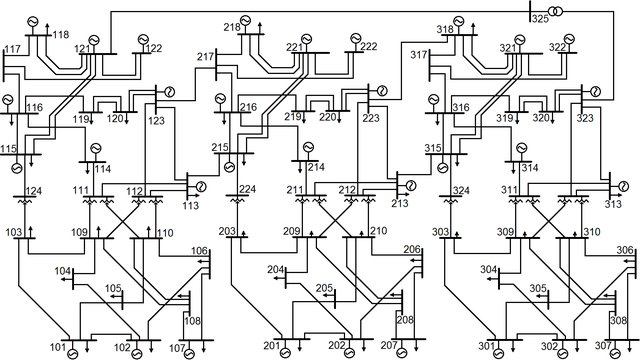
\includegraphics[width=0.8\linewidth]{Figs/RTS.jpg}
    \caption{Reliability test system~\cite{RTS-figure}}
    \label{fig:rts}
\end{figure}

The following dynamic data have been added to those systems. Synchronous generators are represented with a seventh order model. For most generators, the excitation system is represented by an IEEET1 model, and the governor is represented with BPA GG (also known as WSCC type G) model as in~\cite{excitationAndGovernorModels}. A different model is however used for hydro units as they have a fundamentally different behaviour than other types of units. The model used is an GOVHYDRO1 model. Most parameters are taken from annex D of~\cite{vittalBook}. This annex contains typical data for different types of machines (hydro, nuclear, coal, gas) and a wide range of rated powers (5~MW to 1.3~GW). So, for each generators of the test systems, parameters were taken from a machine in~\cite{vittalBook} that has the same type and that has the closest rated power. For hydro units, those parameters are completed with the ones in~\cite{hydroGov}. Models of wind and solar plants still have to be defined. However, WECC models or the generic inverted-connected generation model proposed in~\cite{ChaspierreThesis} will probably be used. Protection models are discussed in chapter~\ref{ch:protections}.

\TODO{Check this 7th order stuff if I have the time, or say ``four winding model" model (one field winding, one d-axis damper winding and two q-axis damper windings) according to Dynawo terminology.}

'Subsequent analysis is required to understand and mitigate high
numbers of unsuccessful simulations'\cite{EurostagHPC}


\TODO{robustness analysis even if out of scope of ``purely-probabilistic" assessment. E.g. redo analysis with all loads increases by 10\% (but with lower statistical accuracy requirements)}

% \cite{TestSystemHenneaux} % for RTS modifications to be N-1 secure

% \subsection{RBTS}
% \label{sec:RBTS}

% will be modernised by decreasing coal capacity (and replace by gas) and add RES in distrib.

% \subsection{GMLC-RTS}